\documentclass{article}
\usepackage{graphicx} % include figures
\usepackage{xeCJK} % Chinese language support
\usepackage{bm}
\usepackage{amsmath,amsthm,amssymb,amsfonts}
\usepackage{cite}
\usepackage[colorlinks,linkcolor=red,anchorcolor=blue,citecolor=green,CJKbookmarks=true]{hyperref}
\usepackage{indentfirst} % indent before a paragraph, Chinese-style
\usepackage{amsmath}
\usepackage[margin=3.5cm]{geometry}
\usepackage{titlesec}
\usepackage{amsmath}
\usepackage{amssymb}
% \linespread{1.6}
\geometry{left=3.2cm,right=3.2cm,top=3.2cm,bottom=3.2cm}
\usepackage{booktabs}
\usepackage{multirow}
\usepackage{array} % assign height for tables
\usepackage{listings}
\usepackage{xcolor}
\usepackage{ulem}
\usepackage{enumitem}
\usepackage{tikz}
\usepackage{lipsum}
\usepackage{empheq} % enable eq numbering inside a brace
\usepackage{float} % forces figs to appear precisely at the location in code
\usepackage[section]{placeins} % prevents figs appearing after its section

\usepackage{mdframed} % when codes cross pages, this is used to add a frame
\setenumerate[1]{itemsep=0pt,partopsep=0pt,parsep=\parskip,topsep=5pt}
\setitemize[1]{itemsep=0pt,partopsep=0pt,parsep=\parskip,topsep=5pt}
\setdescription{itemsep=0pt,partopsep=0pt,parsep=\parskip,topsep=5pt}
% therom
\makeatletter
\thm@headfont{\sc}
\makeatother
\newtheorem{theorem}{Theorem}

\usepackage{hyperref}% keeps internal links (include table of contents) black
\hypersetup{%
  colorlinks = true,
  linkcolor  = black
}

%%%%%%%%%%%%% MATLAB configuration %%%%%%%%%%%%%
%\usepackage{listings} % used for code highlight
%\lstset{extendedchars=false}%这一条命令可以解决代码跨页时,章节标题,页眉等汉字不显示的问题
%\usepackage[framed,numbered,autolinebreaks]{mcode}
\usepackage[T1]{fontenc}
\usepackage[numbered,framed]{matlab-prettifier}
\usepackage{filecontents}
\let\ph\mlplaceholder % shorter macro
\lstMakeShortInline"
\lstset{
  style              = Matlab-editor,
  basicstyle         = \mlttfamily,
  escapechar         = ",
  mlshowsectionrules = true,
}
%\begin{filecontents*}{/code/LIP_straightline.m}

%%%%%%%%%%%% MATLAB configuration %%%%%%%%%%%%%%

%\setCJKmainfont[BoldFont = 黑体]{宋体}
%\setlength{\parindent}{2em} %设置段首空两格
%如果不要缩进 用\noindent

%%%%%%%%%%%%%%%%%%%%%%%%%%%%%%%%%%%%%%%%%%%%%%%%%%%%%%%%%%%%%%%%%%%%%%%%
%%%%%%%%%%%%%%%%%%%%%%%%%%%%%%%%%%%%%%%%%%%%%%%%%%%%%%%%%%%%%%%%%%%%%%%%
%%%%%%%%%%%%%%%%%%%%%%%%%%%%%%%%%%%%%%%%%%%%%%%%%%%%%%%%%%%%%%%%%%%%%%%%
%%%%%%%%%%%%%%%%%%%%          Article             %%%%%%%%%%%%%%%%%%%%%%
%%%%%%%%%%%%%%%%%%%%%%%%%%%%%%%%%%%%%%%%%%%%%%%%%%%%%%%%%%%%%%%%%%%%%%%%
%%%%%%%%%%%%%%%%%%%%%%%%%%%%%%%%%%%%%%%%%%%%%%%%%%%%%%%%%%%%%%%%%%%%%%%%
%%%%%%%%%%%%%%%%%%%%%%%%%%%%%%%%%%%%%%%%%%%%%%%%%%%%%%%%%%%%%%%%%%%%%%%%
\title{ME C134 Lab1 Report}
\author{\large Rui\hspace{0.5cm}Wang\footnote{wangrui@berkeley.edu} \\ 3033461836}
\date{}
\begin{document}
\maketitle
\tableofcontents
\clearpage

\section{General Problem}

  \subsection{Problem Description}
  Given the simple RLC circuit as shown below, we can derive its transfer function as well as state space representation.
        \begin{figure}[H]
        \centering
        \noindent\makebox[\textwidth][c] 
        {
        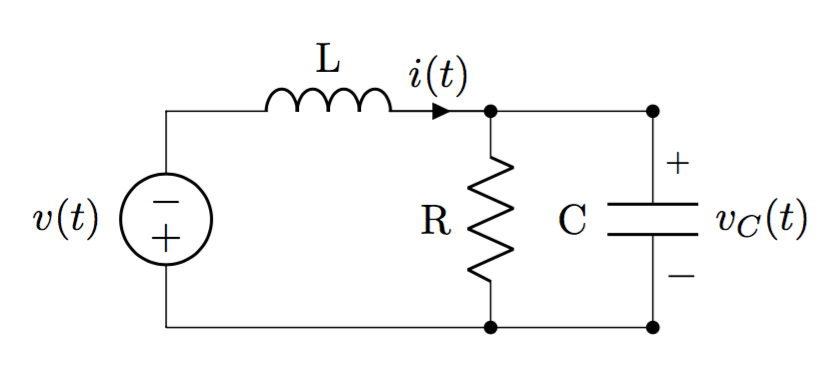
\includegraphics[width=0.3\paperwidth]{images/circuit.png}
        }
        \caption{The original problem: a simple RLC circuit} \label{fig:circuit}
      \end{figure}
  The problem defines $v(t)$ as the input, $i(t)$ and $v_c(t)$ as system states, and $v_c(t)$ as the output.
  
  \subsection{Solution}
   Applying Kirchoff's law (specifically, KVL), we obtain the following equations:
%   $$\left\{
%        \begin{array}{ll}
%           \begin{equation}\label{eq1}
%             L\frac{di(t)}{dt} + v_c(t) + v(t) = 0
%           \end{equation}}\\
%           \begin{equation}\label{eq2}
%             (i(t) - C\frac{dv_c}{dt})R = v_c
%           \end{equation}
%        \end{array}
%   \right.$$\par
   \begin{empheq}[left=\empheqlbrace]{align}
     (i(t) - C\frac{dv_c}{dt})R = v_c \label{eq1}\\
     L\frac{di(t)}{dt} + v_c(t) + v(t) = 0 \label{eq2}
   \end{empheq}
  Differentiate both sides of \eqref{eq1}, and we get 
  \begin{equation}\label{eq3}
    \dot{i} = \frac{\dot{v_c}}{R} + C\ddot{v_c}
  \end{equation}
  Substitute \eqref{eq3} into \eqref{eq1}, and we obtain
  \begin{equation}\label{eq4}
    L(\frac{\dot{v_c}}{R} + C\dot{v_c}) + v_c - v = 0
  \end{equation}
  Therefore, the transfer function turns out to be 
  \begin{equation} \label{eq5}
    \boxed{F(s) = \frac{1}{LCs^2 + \frac{L}{R}s + 1}}
  \end{equation}\par
  Also, rearrange the equations \eqref{eq1} and \eqref{eq4} in the form of $\dot{X} = AX + Bu$, with $X = [i, v_c]^T$ and $u = v$, and $Y = CX + D$, with $Y = v_c$, we obtain the following values for parameters $A, B, C$ and $D$.
  Eventually, we have
  \fbox{
  $A = 
  \begin{bmatrix}
    0 & -\frac{1}{L} \\
    \frac{1}{C} & -\frac{1}{RC}
  \end{bmatrix}$
  $B = [\frac{1}{L}, 0]^T$, $C = [0, 1]$, $D = 0$
  }

\section{Simulation}

  The simulation is a specific implementation of the general problem proposed above. In our implementation, the value of $R, L$ and $C$ are given and fixed as $$R = 2, L = 10^{-3}, C = 10^{-3}$$

  \subsection{Using MATLAB Built-in ODE Solver}
  \subsubsection{Usage}
  In this simulation method, we use MATLAB's ode45 numerical solution to calculate the evolution of $X$ with time. The usage of the function is \verb+[t, x] = ode45(@f, tspan, x0)+, where \verb+f+ is a differential function following a certain format and \verb+tspan+ is a vector with critical time stamp, \verb+x0+ is the initial condition of $X$ in the differential equation.\par
  \verb+ode45+ requires \verb+f+ to be defined in this format: 
  \begin{lstlisting}
    xdot = f(t, x)
  \end{lstlisting}
  where \verb+t, x+ are time $t$ and state variable $X$, respectively.
  \subsubsection{Code}
  In our implementation, we name \verb+f+ as \verb+RLCdynamics+. The code is a simple implementation of the differential equation \eqref{eq4}. Code of the function is attached below:
  \lstinputlisting[style=Matlab-editor, caption = {RLCdynamics.m}]{code/RLCdynamics.m}
  In MATLAB command window, type
  \lstinputlisting[style=Matlab-editor, caption = Plotting $X$ with regard to $t$]{code/cmd1.m}
  we will obtain the following plot\ref{fig:x-t}:
  \begin{figure}[H]
    \centering
    \noindent\makebox[\textwidth][c] 
    {
    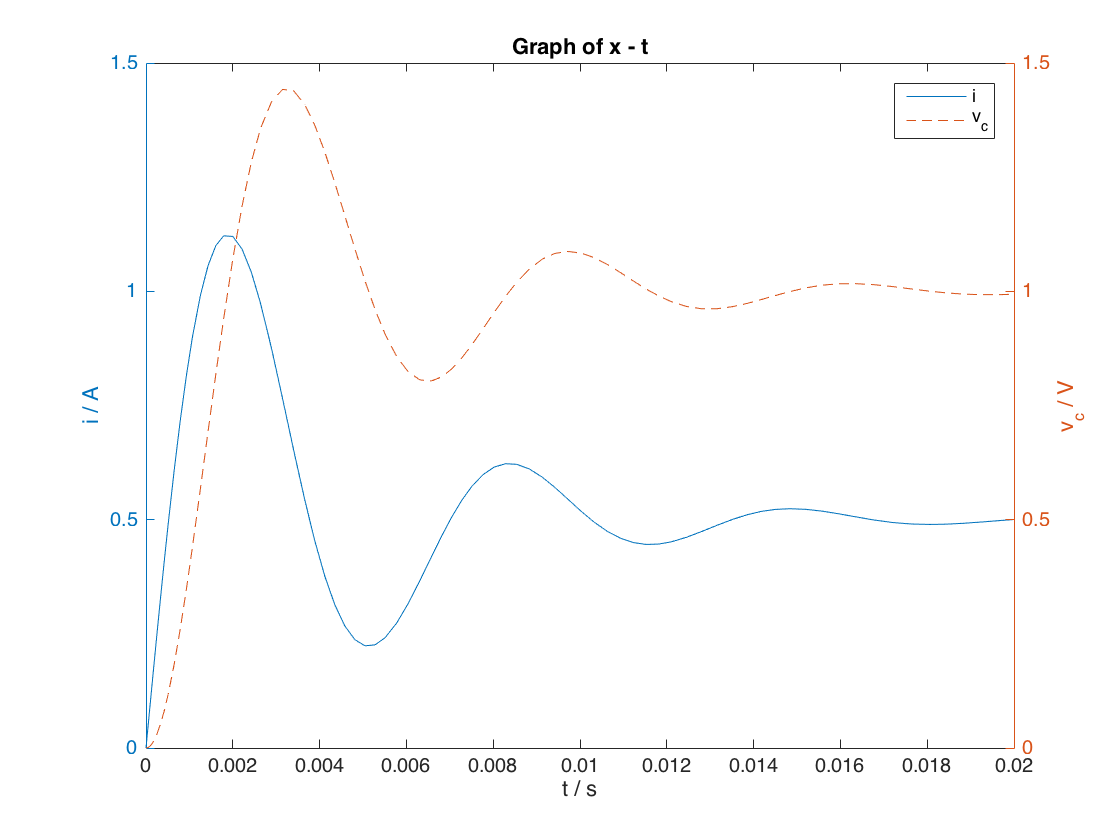
\includegraphics[width=0.5\paperwidth]{images/x-t.png}
    }
    \caption{The evolution of $X$ relative to $t$.} \label{fig:x-t}
  \end{figure}
  \par
  From the plot we can see that both $v_c$ and $i$ follows an underdamped pattern, with their final value stabilized at $1 V$ and $0.5 A$, respectively. This is due to the initial leap by the step input and the later correction(damping) by the circuit(system) itself.

  \subsection{State-space Model}
  \subsubsection{Method}
  This method uses MATLAB's built-in \verb+ss+ function to create a state-space model out of the standard format 
  $$\dot{X} = AX + Bu, Y = CX + Du$$
  \subsubsection{Code}
  \lstinputlisting[style=Matlab-editor, caption = Plotting with state-space model]{code/cmd2.m}\par
  The result is shown below, which is the same as the previous plot, which should be the case as we are modeling the same system, only with different methods.
  \begin{figure}[H]
    \centering
    \noindent\makebox[\textwidth][c] 
    {
    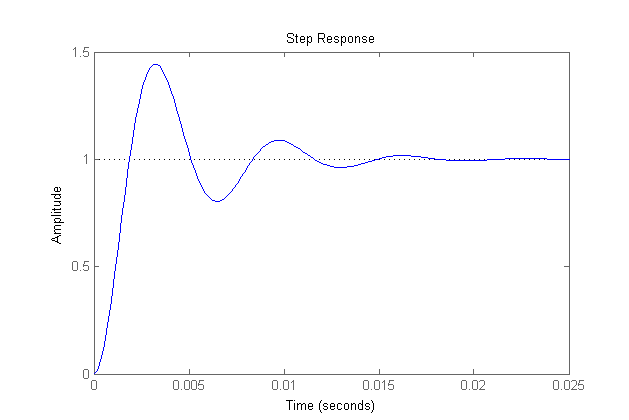
\includegraphics[width=0.4\paperwidth]{images/state_space.png}
    }
    \caption{The evolution of $v_c$ with regard to $t$.} \label{fig:ss}
  \end{figure}
  
  \subsection{Tranfer Function Model}
  \subsubsection{Method}
  In this method, we construct a transfer function and make use of the \verb+step+ function to plot the response of $v_c$.
  \subsubsection{Code}
  \lstinputlisting[style=Matlab-editor, caption = Plotting with transfer function model]{code/cmd3.m}
  \begin{figure}[H]
    \centering
    \noindent\makebox[\textwidth][c] 
    {
    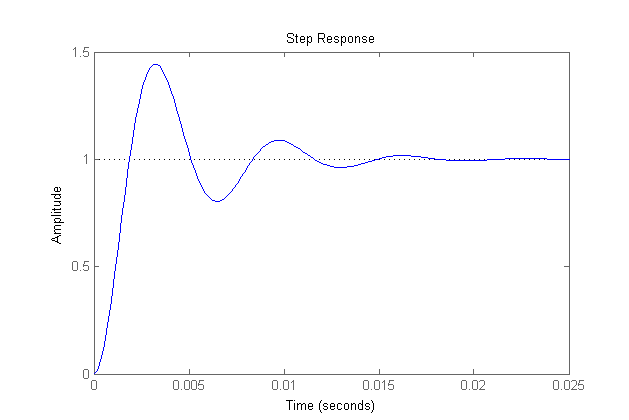
\includegraphics[width=0.4\paperwidth]{images/4.3TF.png}
    }
    \caption{The evolution of $v_c$ with regard to $t$.} \label{fig:tf}
  \end{figure}
  \par
  Basically the three methods above are equivalent, and it is not difficult to understand that their results are the same. In other words, they validate each other.
  
  \subsection{Simulink Model}
  \subsubsection{Method}
  In this method, we construct a Simulink model representing the RLC circuit. As the model for the circuit is not unique, we are given a model architecture and are in charge of the calculation for specific parameters.\par
  \begin{figure}[H]
    \centering
    \noindent\makebox[\textwidth][c] 
    {
    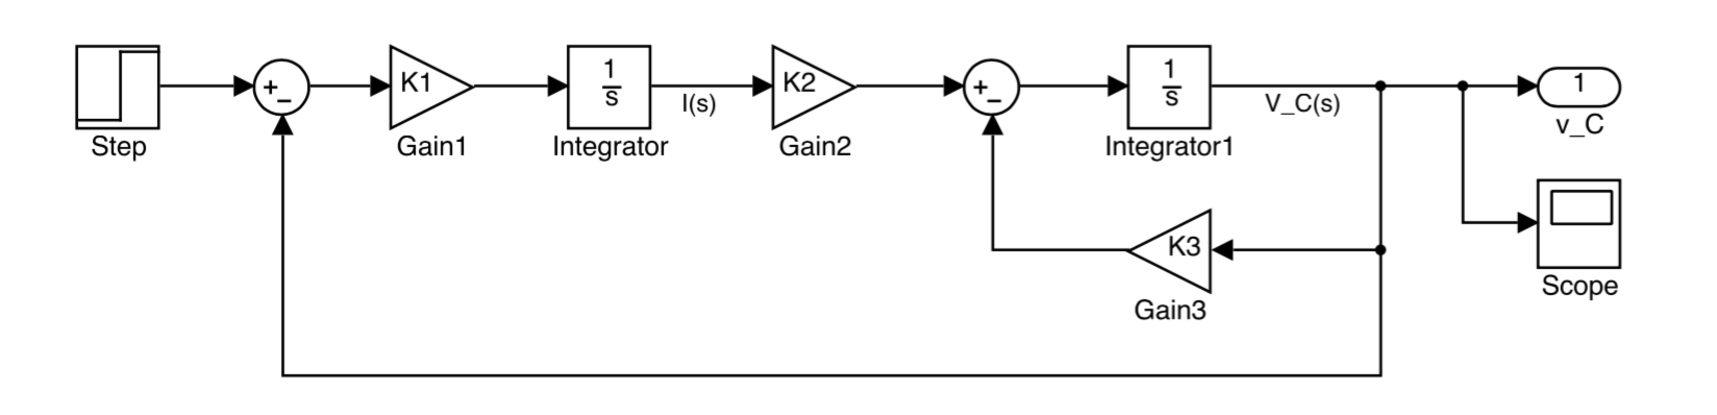
\includegraphics[width=0.5\paperwidth]{images/model0.pdf}
    }
    \caption{The given model.} \label{fig:md0}
  \end{figure}
  We then calculate the parameters $K1, K2$ and $K3$ in the reverse manner:
  \begin{enumerate}
    \item As the output is $v_c$, the value before integration is $\dot{v_c}$, and the value before the first integration is $\ddot{v_c}$ with some coefficient.
    \item According to equation \eqref{eq1}, we have $\dot{v_c} = \frac{i}{C} - \frac{v_c}{RC}$, which enables us to decide that $K3 = \frac{1}{RC}$.
    \item The element directly before and after the first integral can also be decided according to $\dot{v_c} = \frac{i}{C} - \frac{v_c}{RC}$, which is $\dot{i}$ and $i$, respectively.
    \item Furthermore, still with the same equation, we obtain $K2 = \frac{1}{C}$.
    \item According to equation \eqref{eq2}, we have $\dot{i} = \frac{v - v_c}{L}$, which indicates $K1 = \frac{1}{L}$.
    \item Finally, we check whether our derivation is correct by deriving the relationship between variables in the diagram.
  \end{enumerate}\par
  \textbf{Note that the model does not contain differentiation blocks.} \textit{The reason is, instead of using differentiation to obtain values such as $\dot{i}$, we treat them as input and use \textbf{integration} to obtain values such as $v_c$. In the calculation of Simulink model, however, we perform differentiation in order to solve the parameters in the reverse order.}\par
  
  After running the model, we can obtain the evolution of output from data collected by \textbf{scope}. As data in the scope is also stored in MATLAB workspace as \verb+yout+ by default, we can therefore plot the data in MATLAB command window.
  \subsubsection{Model}
  The actual model I constructed looks like this in figure\ref{fig:md}
  \begin{figure}[H]
    \centering
    \noindent\makebox[\textwidth][c] 
    {
    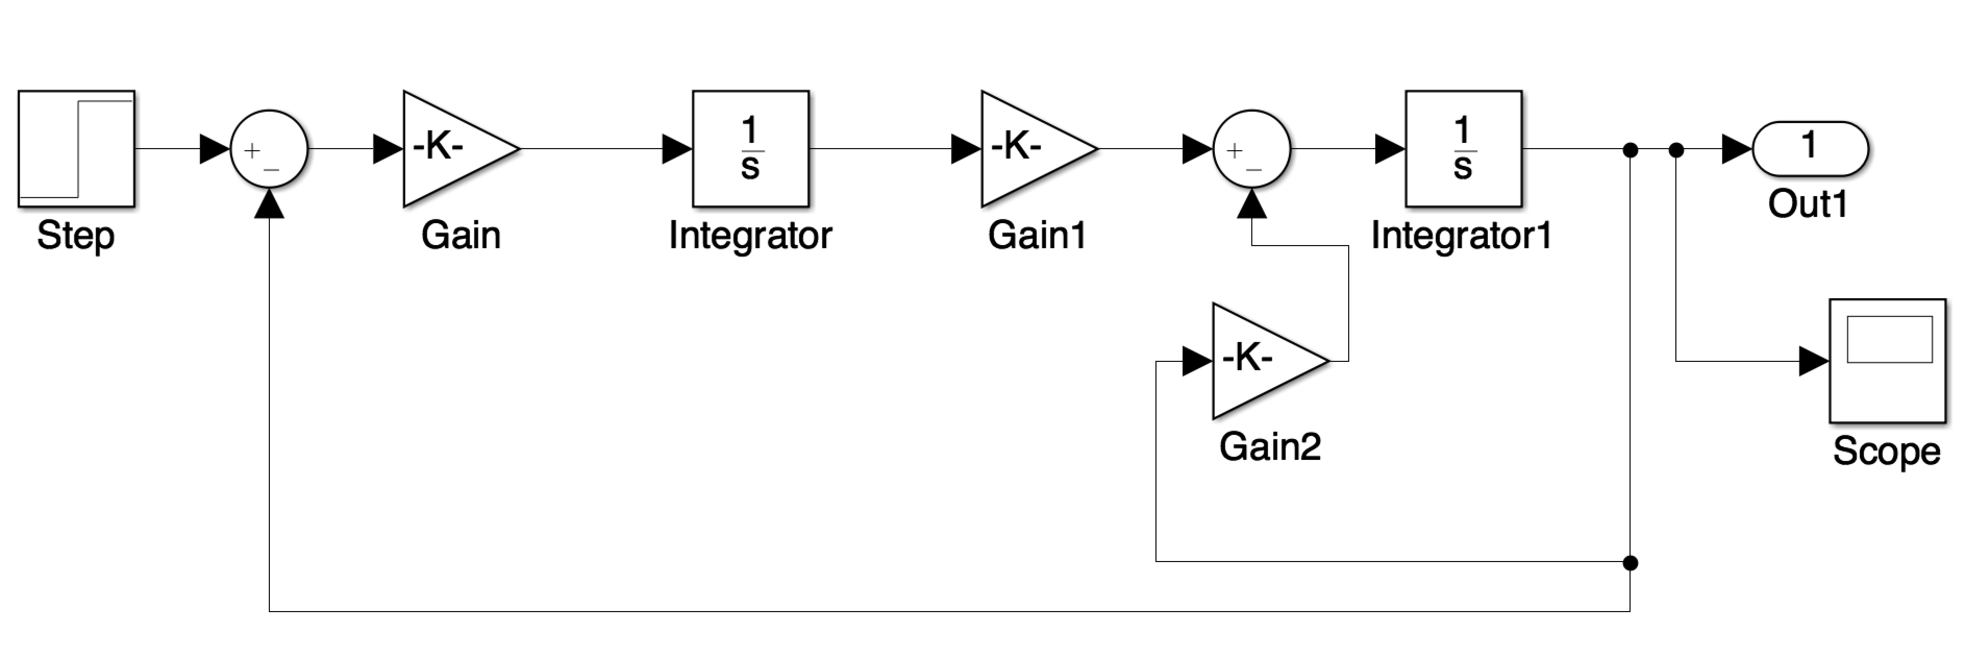
\includegraphics[width=0.46\paperwidth]{images/model.pdf}
    }
    \caption{The final model.} \label{fig:md}
  \end{figure}\par
  Note that on applying the actual data to $K1, K2$ and $K3$, we have $K1 = K2 = 10^3$ and $K3 = 500$.
  
  \subsubsection{Normal Case}
  After configuring Simulink(which is a pain) correctly, we get the following result:
  \begin{figure}[H]
    \centering
    \noindent\makebox[\textwidth][c] 
    {
    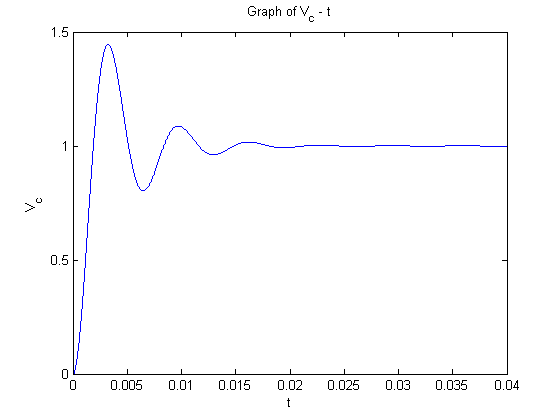
\includegraphics[width=0.4\paperwidth]{images/simulink_plot.png}
    }
    \caption{The Simulink model running result.} \label{fig:sm1}
  \end{figure}
  Again the plot accords with our previous plots, since they are describing the same system.\par
  Following the lab guide, we modify the model input in several ways to see and compare the results. \par
  
  \subsubsection{Changing Initial Condition}
  Changing the initial condition to $1V$, which is to change the initial value of the last integral to $1V$, yields the following result:
  \begin{figure}[H]
    \centering
    \noindent\makebox[\textwidth][c] 
    {
    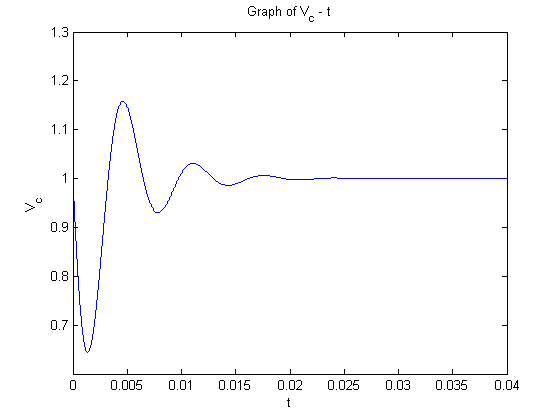
\includegraphics[width=0.4\paperwidth]{images/simu2.png}
    }
    \caption{Initial condition changed to $1 V$.} \label{fig:sm2}
  \end{figure}
  In this case, although the system is at its final state in the beginning, the initial difference at time $0-$ between $v$ and $v_c$ will cause the system to start a dramatic oscillation. However, once oscillation begins, and $v$ is changed to 1 V, the oscillation will be damped. By and by, the system will reach its stability.
  
  \subsubsection{Changing Source to Square Wave}
  To change the input to a square wave, we will need to use the block \textbf{Waveform Generator} and select square wave within the block properties. \textbf{Note} that we also need to select frequency instead of the default "rad/s" as unit.\par
  With a frequency of 25Hz, $v_c$ acts in a periodical pattern, with time interval between the square wave rising/descending trim edge large enough for the output to be damped to stability. This is natural as the square wave for the system is just like a connection of lots of steps, for each step the circuit will act in the same pattern. \textbf{In order to display this periodicity clearly, a $0.12 s$ time span is chosen,} instead of the initial $0.04 s$.
  \begin{figure}[H]
    \centering
    \noindent\makebox[\textwidth][c] 
    {
    \includegraphics[width=0.6\paperwidth]{images/25HZ.png}
    }
    \caption{Input changed to 25Hz square wave.} \label{fig:25hz}
  \end{figure}
  With a frequency of 250Hz, however, input changes too fast for the system to reach stability within a single period. Therefore the system reaches a quasi-stability where it oscillates with the same frequency as the input, which is also called "undamped".
  \begin{figure}[H]
    \centering
    \noindent\makebox[\textwidth][c] 
    {
    \includegraphics[width=0.6\paperwidth]{images/250HZ.png}
    }
    \caption{Input changed to 250Hz square wave.} \label{fig:250hz}
  \end{figure}
  
  \section{Comparison of Different Methods}
  \subsection{Which...Non-linear?}
  \textbf{Which of the model representations above can model non-linear dynamic systems?}\par
  Basically \verb+ode45+ and \textbf{Simulink} are both able to deal with non-linear differential equations. However, in Simulink we have to manually assign the largest step, which is not always easy, especially for very complicated equations. But this does not occur often and Simulink is mostly good enough. The \textbf{state-space model} is designed for linear systems, making it impossible to represent non-linear systems. Modeling using \textbf{transfer function} is also not always viable as for non-linear systems, $X(s)$ and $Y(s)$ can not be factored out from the equation, disabling us from getting a transfer function.\par
  Generally, I think Simulink is the best tool for complicated cases as we do not need to bother with the choice of state variables and the rearrangement of equations.
  
  \subsection{Which...Initial States?}
  \textbf{Which of them is well-suited to account for different initial states?}\par
  Again, both the \textbf{simulate by foot} and \textbf{Simulink} are good, while the other two are not. Because for the former two, initial conditions are treated as variables while for the latter two, initial conditions are not passed in. Instead, we need special functions for each different initial state, which makes life difficult.
  
  \clearpage
  \subsection{Additional Advantages and Disadvantages}
    \begin{table}[htb]
    \setlength{\abovecaptionskip}{0pt}
    \setlength{\belowcaptionskip}{10pt}
    \setlength{\arrayrulewidth}{0.4mm}
    \renewcommand{\arraystretch}{1.5}
    \label{Tab 1}
    \caption{Advantages and Disadvantages of Four Methods}
    \begin{center}
    \begin{tabular}{m{3cm} m{5cm} m{5cm}}
    \hline 
    \hline
    Method & Advantages & Disadvantages\\
    \hline
    %\hline
    Simulate by foot
    & Easy to use in simple cases; optimized and professional, solves quickly
    & Some models can not be solved; needs different solver
      function for different kinds of DE's; requires written-down equations and well-defined variables\\
    Simulink
    & Can model almost anything; graphical and intuitive; does not need writing down equations
    & Needs assigning maximum step; is often not optimized;
      setting-up can be troublesome\\
    State-space Model
    & Clear and general; easily processed by computer
    & Only linear; needs rearrangement and manually performing lots of calculations; matrix can be bulky\\
    Transfer Function Model
    & Can be used to reconstruct system equation easily
    & Only linear; very limited\\
    \hline
    \hline
    \end{tabular}
    \end{center}
    \end{table}
  
% ITEM %
%  Kajita书\textbf{\textit{Introduction to Humanoid Robotics}}第130页给出了LIP的基本流程。
%  \begin{itemize}
%    \item 不变量:每走一步,花的时间是一定的,即$T_{sup}$
%    \item walk parameters $s_x, s_y$的含义是前后两只支撑脚在“每一步”前后的相对位移,而非同一只脚的前后位移
%  \end{itemize}
  
% TABLE %
%    \begin{table}[htb]
%    \setlength{\abovecaptionskip}{0pt}
%    \setlength{\belowcaptionskip}{10pt}
%    \setlength{\arrayrulewidth}{0.4mm}
%    \renewcommand{\arraystretch}{1.5}
%    \label{Tab 1}
%    \caption{Definition of Variables Used in the Code}
%    \begin{center}
%    \begin{tabular}{m{3cm} m{2cm} m{8cm}} % package: array 这个宽度有待调整!
%    \hline 
%    \hline
%    Variable name & Symbol & Meaning\\
%    \hline
%    %\hline
%    zc & $z_c$ & CoM所在平面在z轴的截距,平地上可以认为就是CoM的高度\\%z-axis intersection of CoM's constraint plane \\
%    %\hline
%    Tsup & $T_{sup}$ &机器人每一步的时间 \\
%    \hline
%    \hline
%    \end{tabular}
%    \end{center}
%    \end{table}

%      如图\ref{fig:nostop},如果按照给出的$s_x, s_y$,模拟后我们只能得到

% Code Block %
%      为此我们可以修改程序,把最后的a,b调整为1,1(或者其他合理的比例,使得最后的$(x^d - x_f^{(n)})^2, (\dot{x}^d-\dot{x}_f^{(n)})^2 $都不太大)。
%      \begin{lstlisting}
%        if n == size(sx, 2) - 1 % if time has come to calculate the last step
%          a = 1;
%          b = 1;
%          D = a * (C - 1)^2 + b * (S / Tc)^2;
%        end
%      \end{lstlisting}

\clearpage % print all figures above before new a page
%\appendix
%Appendix:
%
%\lstinputlisting[style=Matlab-editor, caption = {RLCdynamics.m}]{code/RLCdynamics.m}
    %%%%%%%%%%%%%%%
    %%%%%%%%%%%%%%%
    %  CODE HERE  %
    %%%%%%%%%%%%%%%
    %%%%%%%%%%%%%%%
%\lstinputlisting[style=Matlab-editor]{code/RLCdynamics.m}

\end{document}